\dia{Martes 1}{4.5}{%
Un helado cuesta \cent500. Hay una promoci\'on de 6 helados por \cent2500. ?`Cu\'antos helados se pueden comprar con \cent18\,000?
}
{%
Con \cent17\,500 se pueden comprar 42 helados (7 ofertas de 6 helados), y con los \cent500 restantes ser\'ian un total de 43 helados.
}
%%
%%
\dia{Mi\'ercoles 2}{4.5}{%
?`Cu\'antos n\'umeros de d\'igitos distintos, se pueden construir utilizando tres de los d\'igitos 2, 0, 1 y 9?
}{%
  Se tienen 3 posibilidades para el d\'igito de las centenas (el 0 se excluye solo en este caso), 3 para el d\'igito de las decenas y 2 para el d\'igito de las unidades, para un total de $3\times3\times 2=18$ n\'umeros.
}
%%
%%
\dia{Jueves 3}{5.5}{%
Hay 2019 monedas en el ba\'ul izquierdo y el otro est\'a vac\'io. Comenzando hoy se toma todos los d\'ias una moneda del ba\'ul de la izquierda y junto con dos monedas m\'as, se colocan tres monedas en el ba\'ul de la derecha. ?`Llegar\'an a tener el mismo n\'umero de monedas?
}{%
  	}
%%
%%
\dia{Viernes 4}{4.5}{%
Una estrella est\'a formada por un cuadrado y cuatro tri\'angulos equil\'ateros. El per\'imetro del cuadrado es 36\,cm. ?`Cu\'al es el per\'imetro de la estrella? 
}{%
  El cuadrado tiene lado 9\,cm, que es tambi\'en lo que mide el lado de cada tri\'angulo. As\'i, el per\'imetro de la estrella es de 72\,cm.
}
%%
%%
\dia{Lunes 7}{4.5}{%
  Si se sabe que la suma de dos n\'umeros es 2 y su producto es 3, determine la suma del rec\'iproco de dichos n\'umeros.
}{
  Comencemos a partir de lo que se pide calcular:
  \[ \dfrac{1}{x}+\dfrac{1}{y} = \dfrac{x+y}{xy} = \dfrac{2}{3} \]
}
%%
%%
\dia{Martes 8}{4.5}{%
  Se tienen cuatro enteros positivos distintos $a$, $b$, $c$ y $d$. Si $a+b>c+d$ y $b+d=c$, ?`de cu\'antas formas posibles podr\'ian estar ordenados de menor a mayor?
}{%
  Dado que $b+d=c$, se tiene entonces que $c>b$ y $c>d$. Adem\'as, dado que $c>b$ entonces $c+d>b+d$, por lo que $a>d$. As\'i las posibles formas de ordenar son: $b,d,a,c$; $b,d,c,a$; $d,a,b,c$; $d,b,a,c$; $d,b,c,a$.
}
%%
%%
\dia{Mi\'ercoles 9}{4.5}{%
  ?`Ser\'a posible encontrar 5 enteros positivos $\{a,b,c,d,e\}$ tales que ning\'un subconjunto no vac\'io de ellos sea una suma m\'ultiplo de 5?
}{%
  La respuesta es negativa. Supongamos que fuera cierto por un momento, podemos formar entonces los subconjuntos $\{a\}$, $\{a,b\}$, $\{a,b,c\}$, $\{a,b,c,d\}$ y $\{a,b,c,d,e\}$, y la suma de ninguno de tales subconjuntos ser\'ia m\'ultiplo de 5. Tomemos 4 recipientes numerados del 1 al 4, y guardamos el subconjunto que al didivirlo por 5 tiene residuo 1, 2, 3 o 4 en el recipiente respectivo. Como son 5 subconjuntos y 4 recipientes, por el principio del palomar habr\'a dos subconjuntos en el mismo recipiente, tales que el mayor sume $5p+r$ y el menor sume $5q+r$, y como el subconjunto menor est\'a contenido dentro del subconjunto mayor por la forma en que los construimos, al restarlos, nos vamos a quedar con un subconjunto que es divisible por 5.
}
%%
%%
\dia{Jueves 10}{5.5}{%
  El lunes Alejandra env\'ia una foto a 5 amigas. Cada chica que recibe la foto la env\'ia, al d\'ia siguiente, a otras dos amigas que a\'un no la hayan recibido. ?`En qu\'e d\'ia de la semana el n\'umero de chicas que han recibido la foto supera a 100 por primera vez?
}{%
  El martes la foto se env\'ia a 10 nuevas amigas; el mi\'ercoles a 20 nuevas amigas; el jueves a 40 nuevas amigas y el viernes se superan las 100.
}
%%
%%
\dia{Viernes 11}{5.0}{%
  Un triángulo tiene lados de longitud  6, 10 y 11. Un tri\'angulo equil\'atero tiene el mismo per\'imetro que el tri\'angulo original. ?`Cu\'al es la raz\'on de las \'areas del del tri\'angulo original y el tri\'angulo equil\'atero?
}{%
  Usando la f\'ormula de Her\'on se tiene que el semiper\'imetro es $s=27/2$, as\'i que el \'area del tri\'angulo original es de $\sqrt{(27/2)(15/2)(7/2)(5/2)}=45\sqrt{7}/4$. El tr\'iangulo equil\'atero tiene per\'imetro 27, por lo que cada lado mide $9$, la altura mide $9\sqrt{3}/2$, y el \'area es de $81\sqrt{3}/4$. La raz\'on de las \'areas es de
  $\dfrac{45\sqrt{7}}{4} \div \dfrac{81\sqrt{3}}{4} = \dfrac{5\sqrt{21}}{27}$ \smallskip
}
%%
%%
\dia{Lunes 14}{4.5}{%
Juan hizo un c\'alculo usando los d\'igitos $A$, $B$, $C$ y $D$. ?`Qu\'e d\'igito  representa $B$?
\\[1ex]
\centerline{
\begin{tabular}{cccc}
  & $A$ & $B$ & $C$ \\
  $+$ & $C$ & $B$ & $A$ \\ \hline
  $D$ & $D$ & $D$ & $D$
\end{tabular}
}
}{%
  Observe que debajo de tanto $A + C$ como $C + A$ se tiene $D$, por lo que de $B + B$ no se tiene acarreo. As\'i que $ A+ C = 10D + D$, es decir, $A+C=11$, y $B = 0$.
}
%%
%%
\dia{Martes 15}{5.0}{%
  De la lista 3, 5, 2, 6, 1, 4, 7 Marta escoge 3 n\'umeros que suman 8.  De la misma lista Diana escoge 3 n\'umeros que suman 7. ?`Cu\'antos n\'umeros de la lista fueron escogidos tanto por Marta como por Diana?
}{%
  Marta pudo haber escogido $1+2+5$ o $1+3+4$. Diana solo pudo haber escogido $1+2+4$. No importa la escogencia de Marta, siempre se tienen dos n\'umeros en com\'un que tuvieron que ser escogidos por ambas.
}
%%
%%
\dia{Mi\'ercoles 16}{4.5}{%
  La suma de las edades de Karina y su mam\'a es 36. La suma de las edades de la mam\'a y la abuela de Karina es 81. Cuando Karina naci\'o, ?`qu\'e edad ten\'ia su abuela?
}{%
  Se tiene que $K + M=36$ y que $M + A=81$. Si restamos a la segunda ecuaci\'on la primera, nos queda que $A-K=45$. Es decir que la edad de la abuela menos la edad de Karina es 45, que corresponde a la edad que ten\'ia la abuela cuando naci\'o Karina.
} %%
%%
\dia{Jueves 17}{5.2}{%
  Nicol\'as desea repartir los n\'umeros 2, 3, 4, 5, 6, 7, 8, 9 y 10 en varios grupos, de modo que las sumas de los n\'umeros en cada grupo sean todas iguales. ?`Cu\'al es el mayor n\'umero de grupos que Nicol\'as puede formar?
}{%
  Los n\'umeron suman $54=2\cdot 3^3$. Dado que el mayor n\'umero es 10, pueden ser a lo sumo 5 grupos. El m\'aximo divisor de 54 menor o igual que 5 es 3. Es decir, se pueden hacer como m\'aximo 3 grupos, donde cada cual sume 18.
}
%%
%%
\dia{Viernes 18}{5.2}{%
  ?`Cu\'al es la distancia entre los centros de las dos circunferencias?  \\[2ex]
\centerline{
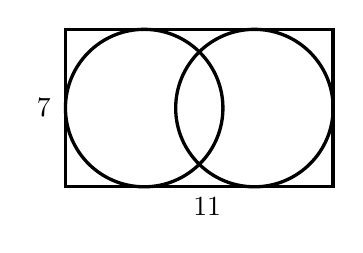
\begin{tikzpicture}[very thick,scale=0.4]
\draw (1,0) rectangle (9.5,5);
\draw (0,2.5) node [left=-10] {7};
\draw (5.5,0) node [below] {11};
\draw (3.5,2.5) circle (2.5);
\draw (7,2.5) circle (2.5);
\end{tikzpicture}
}
}{%
  El radio de las circunferencias es de $3.5$. Observe que la distancia horizontal son dos radios m\'as la distancia entre los centros de los dos c\'irculos. Como los dos radios miden 7, entonces la distancia entre los dos c\'irculos es de 4.
}
%%
%%
\dia{Lunes 21}{5.5}{%
En cada casilla de un tablero de $5\times 5$ se escribe un 1 o un 0, de modo tal que  cada cuadrado de $2\times 2$ contenga exactamente tres n\'umeros iguales. Si se suman todos los n\'umeros en el tablero, ?`cu\'al es el mayor resultado que se puede obtener? 
}{%
  El m\'aximo valor es 21, que corresponde al tablero lleno de unos, a excepci\'on de las 4 casillas que est\'an diagonal a las 4 casillas de las esquinas del tablero.
}
%%
%%
\dia{Martes 22}{6.5}{%
  Se desea escribir los n\'umeros 3, 4, 5, 6, 7, 8 y 9 en los siete c\'irculos, de modo que se obtengan sumas iguales a lo largo de cada una de las tres l\'ineas. ?`Cu\'al es la suma de todos los posibles valores que se pueden colocar en el lugar del signo de interrogaci\'on? \\[1ex]
\centerline{
  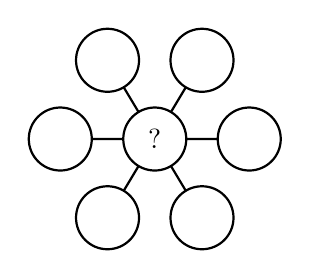
\begin{tikzpicture}[thick,scale=0.4]
    \draw 
    (-1.5,2.5) -- (1.5,-2.5)
    (1.5,2.5) -- (-1.5,-2.5)
    (-3,0) -- (3,0)
    ;
    \filldraw[fill=white] 
    (-3,0) circle[radius=1]
    (-1.5,2.5) circle[radius=1]
    (1.5,2.5) circle[radius=1]
    (3,0) circle[radius=1]
    (1.5,-2.5) circle[radius=1]
    (-1.5,-2.5) circle[radius=1]
    (0,0) circle[radius=1]
    (0,0) node {?}
    ;
  \end{tikzpicture}
}
}{%
  Como el centro es com\'un a todos, entonces se puede quitar de todas las l\'ineas, por lo que nos quedan tres parejas de c\'irculos. La suma de todos los n\'umeros es un m\'ultiplo de 3, as\'i que si colocamos un m\'ultiplo de 3 en el centro, la suma del resto ser\'a m\'ultiplo de 3, y se podr\'an acomodar el resto como se solicita. Es decir, la suma de los posibles valores es $3+6+9=18$.
}
%%
%%
\dia{Mi\'ercoles 23}{5.75}{%
  Un rect\'angulo est\'a dividido en 40 cuadrados id\'enticos. El rect\'angulo contiene m\'as de una fila de cuadrados. Andr\'es ubic\'o la fila de cuadrados del medio (es decir, arriba y abajo hab\'ia el mismo n\'umero de filas) y los pint\'o de colores. ?`Cu\'antos cuadrados dej\'o sin colorear?
}{%
  Se tiene que el n\'umero de filas es un n\'umero impar, as\'i que la \'unica posibilidad es que sean 5 filas (que es el \'unico n\'umero impar que es divisor de 40). As\'i se colorearon 8 cuadrados, y quedaron 32 sin pintar.
}
%%
%%
\dia{Jueves 24}{5.5}{%
  Felipe quiere saber el peso de un libro con una precisi\'on de medio gramo. Sus balanzas solo pesan con precisi\'on de 10 gramos. ?`Cu\'al es el menor n\'umero de copias id\'enticas del libro que Felipe deber\'ia pesar juntas para poder pesar con la precisi\'on que \'el quiere?  
}{%
  El error de la balanza se divide entre el n\'umero de libros pesados. Sea $n$ el n\'umero de libros. As\'i, se quiere que $10/n = 0.5$, de donde nos queda que $n=20$.
}
%%
%%
\dia{Viernes 25}{5.5}{%
  Cada uno de los lados del cuadrado $ABCD$ mide 3~cm.  Los puntos $M$ y $N$ est\'an sobre  $AD$ y $AB$ de tal manera que $CM$ y $CN$ dividen al cuadrado en tres regiones de igual \'area.  ?`Cu\'al es la longitud de $DM$? \\[1ex]
  \centerline {
    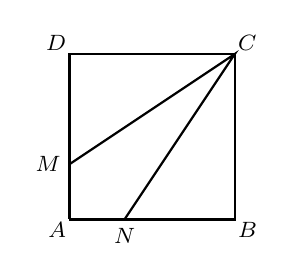
\begin{tikzpicture}[thick,scale=0.7]
      \footnotesize
      \draw (0,0) node [below left=-2] {$A$} -- (3,0) node [below right=-2] {$B$} -- (3,3) node [above right=-2] {$C$} -- (0,3) node [above left=-2] {$D$} -- (0,0);
      \draw (0,1) node [left] {$M$} -- (3,3) -- (1,0) node [below] {$N$};
    \end{tikzpicture}
  }
}{%
  Se tiene que el \'area del cuadrado es 9\,cm$^2$, por lo que cada regi\'on tiene 3\,cm$^2$ de \'area. Si $x$ es la longitud de $DM$, entonces el \'area del $\triangle CDM$ est\'a dada por $3x/2 = 3$, de donde $x=2$\,cm.
}
%%
%%
\dia{Lunes 28}{5.5}{%
  Un le\'on est\'a escondido en una de tres habitaciones. La puerta 1 dice ``El le\'on est\'a aqu\'i''.  La 2 dice ``El le\'on no est\'a aqu\'i''.  La 3 dice ``$2 + 3 = 2 \times 3$''.  Si solo una de las afirmaciones es correcta, ?`en cu\'al habitaci\'on est\'a escondido el le\'on? 
}{%
  Claramente la nota de la habitaci\'on 3 es falsa. As\'i que de las otras dos notas una debe ser verdadera y la otra falsa. La \'unica forma en que eso ocurra, es que el le\'on se encuentre en la habitaci\'on 3.
}
%%
%%
\dia{Martes 29}{5.25}{%
  Alicia escribe una lista de algunos n\'umeros primos menores que 100, usando cada uno  de los d\'igitos  1, 2, 3, 4 y 5 una sola vez y sin usar ning\'un otro d\'igito.  ?`Cu\'al n\'umero primo es seguro que estar\'a en la lista?
}{%
  El 1 no puede estar solo. Los n\'umeros primos que se tienen con el 1 son el 13, el 31 y el 41. Con el 13 y el 31, el 4 no se puede usar con el 2 y el 5 para obtener un n\'umero primo. As\'i que el 41 debe estar en la lista.
}
%%
%%
\dia{Mi\'ercoles 30}{5}{%
  Un hotel afirma que ``!`350 d\'ias de sol todos los a\~nos!''.  De acuerdo a esto, ?`cu\'al es el menor n\'umero de d\'ias que se tiene que estar en el hotel para estar seguro de tener dos d\'ias consecutivos de sol?
}{%
  En el peor de los casos, puede tener un d\'ia de sol, y otro sin sol. Como hay 15 d\'ias sin sol, puede pasar as\'i hasta 30 d\'ias. As\'i, los siguientes dos d\'ias ser\'an de sol. Por lo tanto, se debe estar 32 d\'ias para estar seguro de pasar dos d\'ias consecutivos de sol.
}
%%
%%
\dia{Jueves 31}{5.25}{%
Se escriben los n\'umeros de 1 a 9 en las casillas de un tablero  $3\times 3$.  Luego se calcula la suma de los n\'umeros en cada fila y en cada columna de la tabla.  Cinco de esas sumas, en alg\'un orden, son 12, 13, 15, 16 y 17.  ?`Cu\'al es la sexta? 
}{%
  La suma de los n\'umeros del 1 al 9 es 45. En la tabla, cada n\'umero se suma dos veces, es decir que la suma total es de 90. Al sumar los cinco resultados dados, se tiene un total de 73, por lo que la sexta suma es $90-73=17$.
}
%%
%%
